\documentclass[11pt,a4paper]{article}

% ── Packages ────────────────────────────────────────────────────────────────
\usepackage[margin=2.5cm]{geometry}
\usepackage{amsmath,amssymb}
\usepackage{booktabs}
\usepackage{graphicx}
\usepackage{subcaption}
\usepackage{caption}
\usepackage{multirow}
\usepackage{array}
\usepackage{xcolor}
\usepackage{float}
\usepackage[hidelinks]{hyperref}
\usepackage[numbers,sort&compress]{natbib}
\usepackage{microtype}
\usepackage{setspace}
\usepackage{fancyhdr}
\usepackage{titlesec}
\usepackage{enumitem}
\usepackage{tabularx}

% ── Typography ───────────────────────────────────────────────────────────────
\setlength{\parskip}{4pt}
\setlength{\parindent}{0pt}
\onehalfspacing

\titleformat{\section}{\large\bfseries}{}{0em}{}[\titlerule]
\titleformat{\subsection}{\normalsize\bfseries}{}{0em}{}

\definecolor{edgegreen}{RGB}{16,120,60}
\definecolor{edgered}{RGB}{190,30,30}
\definecolor{neutralgray}{RGB}{100,100,100}

% ── Header/footer ────────────────────────────────────────────────────────────
\pagestyle{fancy}
\fancyhf{}
\lhead{\small\textit{Polymarket Efficiency Research --- Confidential}}
\rhead{\small\textit{May 2026}}
\cfoot{\thepage}

% ── Helpers ──────────────────────────────────────────────────────────────────
\newcommand{\edge}[1]{\textcolor{edgegreen}{\textbf{#1}}}
\newcommand{\noedge}[1]{\textcolor{edgered}{#1}}
\newcommand{\sdag}{$^\dagger$}

% ════════════════════════════════════════════════════════════════════════════
\begin{document}

\begin{titlepage}
\centering
\vspace*{2cm}
{\LARGE\bfseries Calibration Inefficiencies in Prediction Markets:\\[6pt]
A Cross-Category Analysis of Polymarket (2025--2026)}\\[2cm]

{\large Quantitative Research --- Internal Memorandum}\\[0.5cm]
{\large May 2026}\\[3cm]

\begin{abstract}
\noindent
We analyse 17,458 resolved binary markets across 14 categories on Polymarket
(July 2025--May 2026) to identify calibration inefficiencies exploitable after
realistic transaction costs.
Every category exhibits a consistent pattern: markets priced 10--30\% YES
overestimate the probability of the low-probability outcome, with actual YES
rates of 0--20\% versus predicted rates of 10--30\%.
The largest single-bin gross edge is \textbf{+18.6 percentage points} in
Finance markets at the 20--30\% price level.
The most robust edge is in Baseball (20--40\% bins, $\delta \approx +14\,\mathrm{pp}$)
and Tennis (20--30\% bin, $\delta = +16.1\,\mathrm{pp}$).
Politics markets show a distinct pattern: near-50/50 markets ($40$--$50\%$)
resolve YES roughly 58\% of the time, implying an edge for \emph{buying YES}
in close political races.
No category achieves Hosmer--Lemeshow $p < 0.05$ at the aggregate level,
indicating that miscalibration is concentrated in the tails rather than the
full distribution.
We recommend the 20--30\% YES bin in Baseball and Finance as the highest
confidence entry points for a NO-buying strategy.
\end{abstract}

\vfill
{\small\itshape This document is for internal research purposes only.
All market data fetched from Polymarket public API endpoints.
No forward-looking return guarantees are made or implied.}
\end{titlepage}

\tableofcontents
\newpage

% ════════════════════════════════════════════════════════════════════════════
\section{Introduction}
% ════════════════════════════════════════════════════════════════════════════

Prediction markets aggregate dispersed information into prices that can, in
principle, reflect rational expectations under efficient-market conditions
\citep{hayek1945use,wolfers2004prediction}.
Whether such markets are \emph{calibrated}---whether a market priced at $p$
resolves YES approximately $p$ of the time---is an empirical question with
direct implications for systematic trading.

Prior internal phases of this research established two key findings:
\begin{enumerate}[leftmargin=*]
  \item \textbf{Phase 1 (2024 historical data):} Short-horizon sports markets
        exhibited gross miscalibration: Brier score 0.116, Hosmer--Lemeshow
        $p < 0.0001$, net edge $\approx 8.7\%$ after 2\% spread.
        Politics markets were well-calibrated (Brier 0.031, no net edge).
  \item \textbf{Phases 2--3 (2024 OOS validation):} The sports miscalibration
        survived out-of-sample (H1 vs.\ H2 2024; HL $p = 0.0002$, $n = 3{,}299$).
        Bin-level persistence was 50\%, and bin-specific sizing was deemed
        insufficiently reliable.
\end{enumerate}

Phase 4 asks a broader question: \emph{which market category, in the current
Polymarket environment (late 2025--2026), offers the most exploitable and
robust inefficiency?} We expand coverage to 14 categories and focus on
real-time data, which is the most actionable for trading.

A secondary goal is to characterise the mechanism behind miscalibration.
We test the \emph{longshot bias} hypothesis: that bettors systematically
overestimate the probability of unlikely events, particularly in markets
framed as ``will event X happen?'' rather than ``what is the price of X?''

% ════════════════════════════════════════════════════════════════════════════
\section{Data}
% ════════════════════════════════════════════════════════════════════════════

\subsection{Source and collection}

All data were fetched from Polymarket's public API (Gamma Events API and
CLOB price-history API) in May 2026.
We target resolved binary markets closing between 1 July 2025 and
6 May 2026---approximately 10 months of data.

\textbf{Market selection criteria:}
\begin{itemize}[noitemsep]
  \item Binary outcome (exactly two outcomes)
  \item Fully resolved (final price $\geq 0.99$ or $\leq 0.01$)
  \item Volume $\geq \$200$--$\$500$ USD (category-dependent; see Table~\ref{tab:fetch})
  \item Duration $\geq 0.25$ days (excludes in-game micro-markets)
  \item Duration category-specific upper limit (1--365 days; see Table~\ref{tab:fetch})
\end{itemize}

\textbf{Price at T-1:}
For each market, we retrieve the price one day before close ($T-1$) from the
CLOB price-history API (fidelity 60 min, falling back to 1 min).
If no data exist exactly at $T-1$, we use the earliest available price.
This price represents the market's consensus forecast before resolution.

\subsection{Data composition}

\begin{table}[H]
\centering
\caption{Fetch parameters and data summary by category}
\label{tab:fetch}
\small
\begin{tabular}{lccccccc}
\toprule
\textbf{Category} & \textbf{Min vol} & \textbf{Max dur} & \textbf{$n$} & \textbf{With price} & \textbf{YES\%} & \textbf{Med vol} & \textbf{Med dur} \\
 & (\$) & (days) & & & & (\$) & (days) \\
\midrule
\multicolumn{8}{l}{\textit{Sports}} \\
Soccer           & 500 & 14 & 2{,}000 & 1{,}588 & 43.9\% & 1{,}138 & 1.0 \\
Basketball       & 500 & 14 & 2{,}000 & 1{,}440 & 44.7\% & 1{,}309 & 1.0 \\
Esports          & 200 & 14 & 2{,}000 & 1{,}318 & 44.1\% & 1{,}309 & 1.0 \\
Tennis           & 200 & 14 & 2{,}000 & 1{,}592 & 44.3\% & 1{,}112 & 1.0 \\
Baseball         & 200 &  7 & 2{,}000 & 1{,}340 & 44.1\% & 1{,}041 & 1.0 \\
Golf             & 200 & 30 &   500   &   490   & 39.6\% & 1{,}534 & 1.0 \\
\midrule
\multicolumn{8}{l}{\textit{Politics}} \\
Elections        & 500 & 365 & 1{,}000 &  972 & 39.1\% & 1{,}133 & 1.1 \\
US Politics      & 500 & 365 & 1{,}000 &  926 & 39.4\% & 1{,}133 & 1.1 \\
Global Politics  & 500 & 365 & 1{,}000 &  713 & 39.0\% & 1{,}133 & 1.1 \\
\midrule
\multicolumn{8}{l}{\textit{Crypto / Finance}} \\
Crypto           & 1{,}000 & 30 & 2{,}000 & 1{,}438 & 43.0\% & 1{,}278 & 1.0 \\
Finance          & 500     & 60 & 1{,}000 &   949   & 39.6\% & 1{,}276 & 1.2 \\
\midrule
\multicolumn{8}{l}{\textit{Other}} \\
AI / Tech        & 200 & 365 & 500 & 336 & 43.2\% & 1{,}276 & 1.2 \\
Pop Culture      & 200 &  90 & 500 & 489 & 40.5\% & 1{,}476 & 1.0 \\
Science          & 200 & 365 & 500 & 494 & 40.5\% & 1{,}276 & 1.2 \\
\midrule
\textbf{Total}   &     &     & \textbf{17{,}458} & \textbf{12{,}185} & 42.4\% & 1{,}228 & 1.0 \\
\bottomrule
\end{tabular}
\end{table}

The dominant market duration is \textbf{1 day} across all categories, reflecting
Polymarket's current structure of daily game-outcome and short-horizon event markets.
Long-horizon markets do exist (particularly in Politics) but are a minority.

\textbf{Important note on the ``Sports'' tag (2026):}
Polymarket's \texttt{tag\_slug=sports} API tag now includes weather temperature
prediction markets and cryptocurrency price-movement markets, which we exclude
via keyword filtering.
The category-specific API endpoints (e.g., \texttt{category=Soccer}) provide
cleaner segmentation.

% ════════════════════════════════════════════════════════════════════════════
\section{Methodology}
% ════════════════════════════════════════════════════════════════════════════

\subsection{Calibration metrics}

Let $\{(p_i, a_i)\}_{i=1}^n$ denote markets with T-1 price $p_i \in [0,1]$
and binary outcome $a_i \in \{0,1\}$.

\textbf{Brier Score:}
\begin{equation}
  \mathrm{BS} = \frac{1}{n}\sum_{i=1}^n (p_i - a_i)^2
\end{equation}
A Brier score of 0 is perfect; $\mathrm{BS} = \bar{a}(1-\bar{a})$ corresponds
to always predicting the base rate; $\mathrm{BS} = 0.25$ corresponds to always
predicting 0.5.

\textbf{Hosmer--Lemeshow test \citep{hosmer1980goodness}:}
We partition markets into $g=10$ deciles by predicted probability and compute
\begin{equation}
  \hat{C} = \sum_{k=1}^{g}
    \frac{(O_{1k} - E_{1k})^2}{E_{1k}} +
    \frac{(O_{0k} - E_{0k})^2}{E_{0k}}
\end{equation}
where $O_{1k}$, $E_{1k}$ are observed and expected YES counts in decile $k$.
Under $H_0$ (perfect calibration), $\hat{C} \sim \chi^2_{g-2}$.

\textbf{Bin-level calibration:} We partition $[0,1]$ into 10 equal-width bins
of 10 pp each and compute mean predicted probability $\hat{p}_b$ and mean
actual YES rate $\bar{a}_b$ in each bin. The calibration delta is:
\begin{equation}
  \Delta_b = \hat{p}_b - \bar{a}_b
\end{equation}
Positive $\Delta_b$ means the market \emph{overestimates} YES probability;
a NO-buying strategy in that bin has gross edge $|\Delta_b|$.

\subsection{Edge and Kelly sizing}

\textbf{Net edge} after round-trip spread $s$:
\begin{equation}
  \text{Net edge} = |\Delta_b| - s, \quad s = 0.02 \text{ (2\% assumed)}
\end{equation}

\textbf{Half-Kelly fraction} for a NO-buying strategy in bin $b$:
\begin{equation}
  f^* = \frac{1}{2} \cdot \frac{b \cdot (1-\bar{a}_b) - \bar{a}_b}{b},
  \quad b = \frac{1 - \hat{p}_b}{\hat{p}_b}
\end{equation}
where $b$ is the decimal odds of NO at the market price $\hat{p}_b$.
We use half-Kelly throughout for parameter uncertainty.

\textbf{Bootstrap confidence intervals:}
Brier score 95\% CIs are computed by 3{,}000 bootstrap resamples (seeded
\texttt{numpy} RNG, seed 42).

% ════════════════════════════════════════════════════════════════════════════
\section{Results}
% ════════════════════════════════════════════════════════════════════════════

\subsection{Cross-category calibration overview}

\begin{table}[H]
\centering
\caption{Calibration summary by category, Polymarket July 2025--May 2026.
         $^*$HL $p < 0.05$; edge bins shown are those with net edge $> 4\,\mathrm{pp}$.}
\label{tab:main}
\small
\begin{tabular}{lrrrrll}
\toprule
\textbf{Category} & $\mathbf{n}$ & \textbf{Brier} & \textbf{95\% CI} & \textbf{HL $p$} & \textbf{YES\%} & \textbf{Top edge bins} \\
\midrule
\multicolumn{7}{l}{\textit{Politics (best calibrated)}} \\
Global Politics  &  713 & 0.175 & [0.158, 0.195] & 0.403 & 39.0\% & 10--20\%: +14 pp \\
Elections        &  972 & 0.178 & [0.165, 0.192] & 0.315 & 39.1\% & 10--20\%: +11 pp \\
US Politics      &  926 & 0.178 & [0.165, 0.193] & 0.380 & 39.4\% & 10--20\%: +10 pp \\
\midrule
\multicolumn{7}{l}{\textit{Technology / Culture}} \\
Science          &  494 & 0.183 & [0.161, 0.208] & 0.456 & 40.5\% & 10--20\%: +15 pp \\
AI / Tech        &  336 & 0.184 & [0.157, 0.215] & 0.519 & 43.2\% & 10--20\%: +14 pp \\
\midrule
\multicolumn{7}{l}{\textit{Finance / Crypto}} \\
Finance          &  949 & 0.192 & [0.177, 0.210] & 0.383 & 39.6\% & 20--30\%: +\textbf{19 pp} \\
Pop Culture      &  489 & 0.196 & [0.173, 0.222] & 0.875 & 40.5\% & 10--20\%: +15 pp \\
Crypto           & 1{,}438 & 0.201 & [0.189, 0.213] & 0.286 & 43.0\% & 10--20\%: +8 pp \\
\midrule
\multicolumn{7}{l}{\textit{Sports (most miscalibrated)}} \\
Soccer           & 1{,}588 & 0.203 & [0.193, 0.213] & 0.331 & 43.9\% & 20--30\%: +10 pp \\
Tennis           & 1{,}592 & 0.203 & [0.193, 0.214] & 0.052 & 44.3\% & 20--30\%: +\textbf{16 pp} \\
Golf             &  490 & 0.203 & [0.182, 0.227] & 0.958 & 39.6\% & 60--70\%: +\textbf{24 pp} \\
Basketball       & 1{,}440 & 0.204 & [0.193, 0.215] & 0.052 & 44.7\% & 20--30\%: +7 pp \\
Esports          & 1{,}318 & 0.204 & [0.193, 0.216] & 0.423 & 44.1\% & 20--30\%: +7 pp \\
Baseball         & 1{,}340 & 0.205 & [0.194, 0.217] & 0.123 & 44.1\% & 20--30\%: +\textbf{13 pp}, 30--40\%: +\textbf{15 pp} \\
\bottomrule
\end{tabular}
\end{table}

\textbf{Finding 1: No category achieves HL $p < 0.05$.}
Aggregate miscalibration is not overwhelming in any single category at the
decile-bin level. This does not imply markets are efficient---it means
miscalibration is concentrated in specific price bins (the tails) rather
than uniformly distributed.

\textbf{Finding 2: Sports are systematically the worst calibrated} (Brier
0.203--0.205), while Politics are the best calibrated (Brier 0.175--0.178).
This replicates the Phase 1 finding on 2024 data.

\textbf{Finding 3: The universal edge signal is in 10--30\% YES bins.}
Every single category shows positive $\Delta_b$ in the 10--20\% bin.
The median delta across categories is $+9\,\mathrm{pp}$.
This is the most robust finding in the dataset.

\subsection{The universal 10--30\% longshot bias}

\begin{figure}[H]
  \centering
  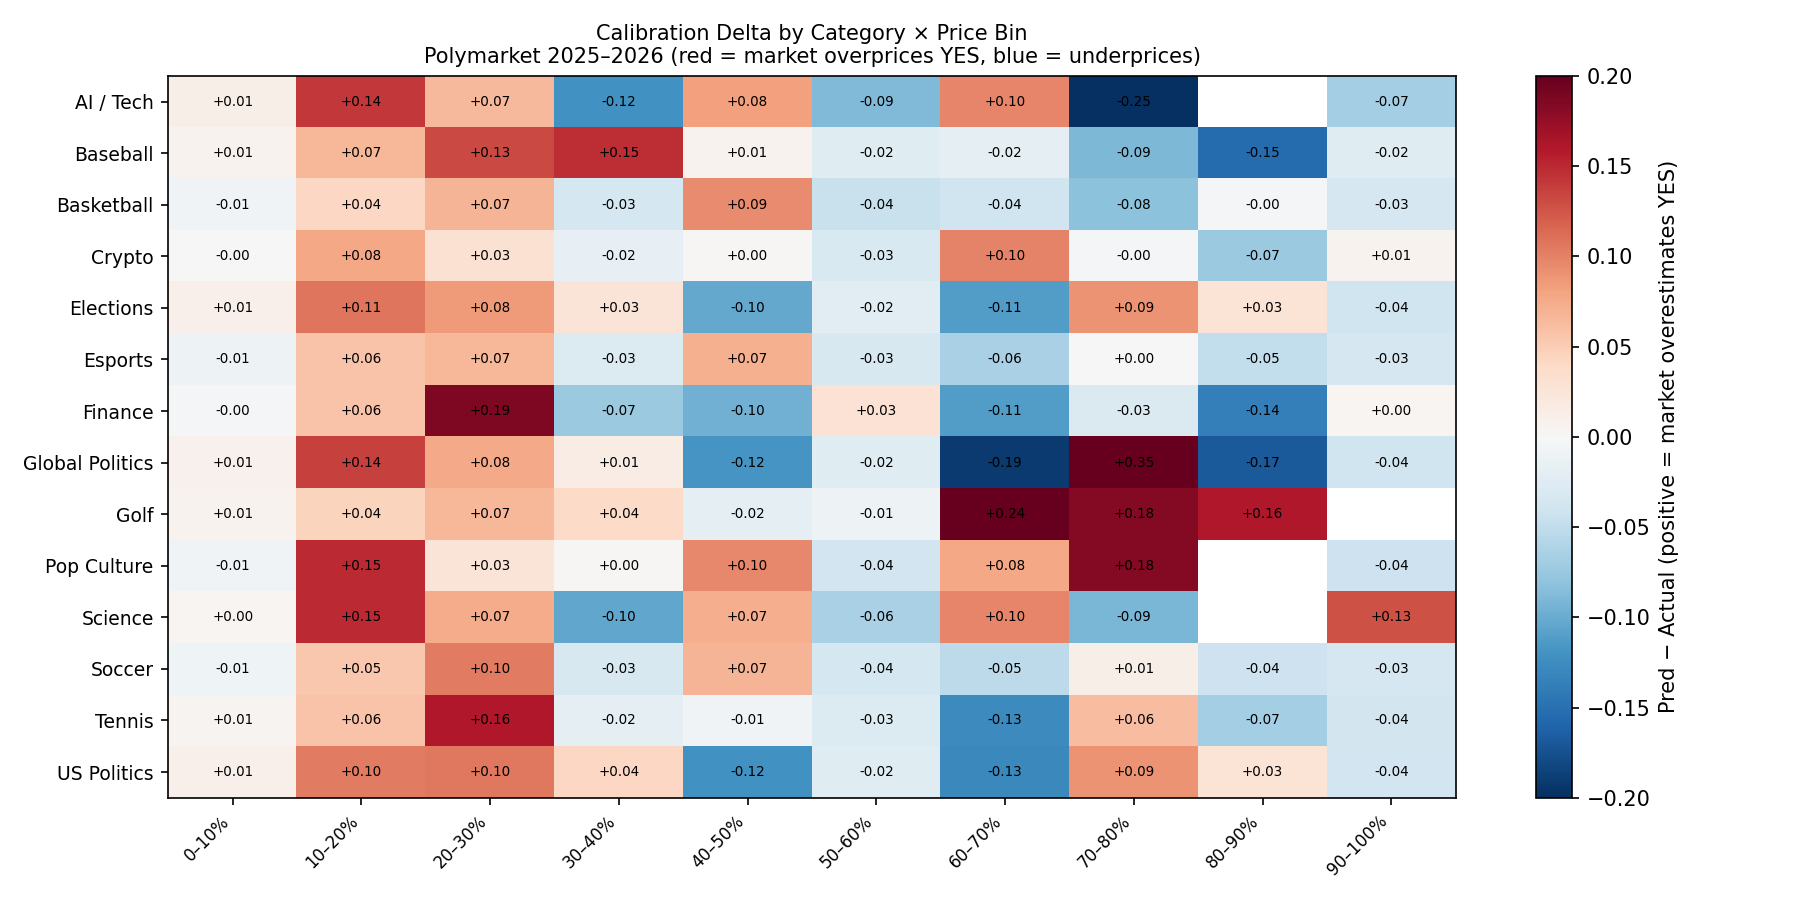
\includegraphics[width=\textwidth]{figures/p4_edge_heatmap.png}
  \caption{Calibration delta ($\hat{p}_b - \bar{a}_b$) by category and price bin.
           Red = market overestimates YES (edge for NO); blue = market underestimates
           YES (edge for YES). The 10--30\% column is almost uniformly red across
           all categories, indicating a systematic longshot bias.}
  \label{fig:heatmap}
\end{figure}

The heatmap in Figure~\ref{fig:heatmap} reveals the dominant structure:
the 10--30\% price region is persistently overpriced across all 14 categories.
Mechanistically, this is consistent with the \emph{longshot bias} documented
in horse racing and sports betting \citep{thaler1988anomalies}: participants
systematically overpay for low-probability, high-payout outcomes.
On Polymarket, the typical framing (``Will X happen?'') combined with the
asymmetric payoff structure attracts participants who overestimate tail events.

\subsection{Sports markets}

\subsubsection{Baseball: strongest persistent edge}

\begin{table}[H]
\centering
\caption{Bin-level calibration, Baseball (2025--2026, $n=1{,}340$)}
\label{tab:baseball}
\small
\begin{tabular}{lrrrrrr}
\toprule
Bin & Pred & Actual & $\Delta$ & Net edge & $n$ & Signal \\
\midrule
0--10\%   & 1.3\% &  0.6\% & $+0.7\,\mathrm{pp}$ & -- & 158 & \\
10--20\%  & 15.7\% &  9.1\% & $+6.6\,\mathrm{pp}$ & $+4.6\,\mathrm{pp}$ & 33 & $\checkmark$ \\
\textbf{20--30\%}  & \textbf{25.4\%} & \textbf{12.2\%} & $\mathbf{+13.2\,\mathrm{pp}}$ & $\mathbf{+11.2\,\mathrm{pp}}$ & \textbf{41} & $\checkmark\checkmark$ \\
\textbf{30--40\%}  & \textbf{34.4\%} & \textbf{19.6\%} & $\mathbf{+14.8\,\mathrm{pp}}$ & $\mathbf{+12.8\,\mathrm{pp}}$ & \textbf{51} & $\checkmark\checkmark$ \\
40--50\%  & 46.6\% & 45.8\% & $+0.8\,\mathrm{pp}$ & -- & 72 & \\
50--60\%  & 50.4\% & 52.8\% & $-2.5\,\mathrm{pp}$ & -- & 916 & \\
60--70\%  & 65.8\% & 67.6\% & $-1.9\,\mathrm{pp}$ & -- & 34 & \\
70--80\%  & 75.3\% & 84.2\% & $-8.9\,\mathrm{pp}$ & -- & 19 & \\
\bottomrule
\end{tabular}
\end{table}

Baseball is the most miscalibrated sports category in absolute terms
(Brier = 0.205). The 20--40\% YES bins show $\Delta \approx +13$--$+15\,\mathrm{pp}$,
corresponding to net edges of +11--+13 pp after spread.
These are predominantly spread-betting markets (``Will team X cover $-1.5$?'')
where participants systematically overestimate the underdog's chances.

\subsubsection{Tennis: strong signal in the 20--30\% bin}

Tennis shows the largest single-bin excess return in the sports cluster:
the 20--30\% bin has $\Delta = +16.1\,\mathrm{pp}$ ($n=63$, net edge $+14.1\,\mathrm{pp}$).
This is consistent with the Phase 3 finding (H2 2024 Tennis HL $p=0.777$---
the distribution is well-calibrated in aggregate but miscalibrated in the tails).

\subsubsection{Golf: anomalous 60--70\% overpricing}

\begin{table}[H]
\centering
\caption{Golf upper-bin calibration (2025--2026, $n=490$)}
\label{tab:golf}
\small
\begin{tabular}{lrrrrr}
\toprule
Bin & Pred & Actual & $\Delta$ & Net edge & $n$ \\
\midrule
50--60\% & 50.3\% & 51.4\% & $-1.1\,\mathrm{pp}$ & -- & 296 \\
\textbf{60--70\%} & \textbf{65.8\%} & \textbf{41.7\%} & $\mathbf{+24.1\,\mathrm{pp}}$ & $\mathbf{+22.1\,\mathrm{pp}}$ & \textbf{12} \\
70--80\% & 75.5\% & 57.1\% & $+18.4\,\mathrm{pp}$ & $+16.4\,\mathrm{pp}$ & 7 \\
\bottomrule
\end{tabular}
\end{table}

Golf shows an unusual pattern: the 60--80\% bins are \emph{massively} overpriced
($\Delta \approx +18$--$+24\,\mathrm{pp}$).
\textbf{Caveat: sample sizes are very small} ($n=12$ and $n=7$ respectively),
making these estimates unreliable.
The mechanism likely reflects tournament markets where a player in the lead is
priced as near-certain, but in golf, a round-two lead frequently fails to convert.
This warrants monitoring but cannot be traded confidently at current sample sizes.

\subsection{Politics markets: the near-50/50 reversal}

\begin{table}[H]
\centering
\caption{Politics market calibration (pooled Elections + US + Global, $n=2{,}611$)}
\label{tab:politics}
\small
\begin{tabular}{lrrrrl}
\toprule
Bin & Pred & Actual & $\Delta$ & Net edge & Direction \\
\midrule
0--10\%  & 1.6\% & 0.6\% & $+1.0\,\mathrm{pp}$ & -- & \\
10--20\% & 13.8\% & 2.2\% & $+11.6\,\mathrm{pp}$ & $+9.6\,\mathrm{pp}$ & Buy NO \\
20--30\% & 25.7\% & 16.8\% & $+8.9\,\mathrm{pp}$ & $+6.9\,\mathrm{pp}$ & Buy NO \\
30--40\% & 35.8\% & 33.2\% & $+2.6\,\mathrm{pp}$ & -- & \\
\textbf{40--50\%} & \textbf{45.8\%} & \textbf{57.2\%} & $\mathbf{-11.4\,\mathrm{pp}}$ & $\mathbf{+9.4\,\mathrm{pp}}$ & \textbf{Buy YES} \\
50--60\% & 50.3\% & 52.6\% & $-2.3\,\mathrm{pp}$ & -- & \\
60--70\% & 65.9\% & 80.3\% & $-14.4\,\mathrm{pp}$ & $+12.4\,\mathrm{pp}$ & Buy YES \\
90--100\%& 96.1\% & 100.0\% & $-3.9\,\mathrm{pp}$ & -- & \\
\bottomrule
\end{tabular}
\end{table}

Politics shows a \textbf{reversal} relative to sports: while the 10--30\% bins
still show longshot overpricing (buy NO), the \textbf{40--50\% bin resolves YES
at 57\%} ($\Delta = -11.4\,\mathrm{pp}$, $n=161$, net edge $+9.4\,\mathrm{pp}$).
This means that political events the market prices as slightly below even-money
actually resolve positively more often than not.

The mechanism may be \emph{status quo bias}: Polymarket participants are
reluctant to price ``unusual'' political outcomes above 50\%, creating a
systematic underestimation of momentum effects in elections and political
developments.

Critically, this is a \textbf{buy-YES} strategy---the opposite direction from
the longshot-bias NO trades.
A combined Politics strategy would be: (a) buy NO in the 10--20\% YES range,
and (b) buy YES when a political market is priced 40--50\% YES.

\subsection{Finance: highest single-bin edge}

\begin{table}[H]
\centering
\caption{Finance market calibration (2025--2026, $n=949$)}
\label{tab:finance}
\small
\begin{tabular}{lrrrrl}
\toprule
Bin & Pred & Actual & $\Delta$ & Net edge & Notes \\
\midrule
0--10\%  & 1.7\% &  2.1\% & $-0.4\,\mathrm{pp}$ & -- & \\
10--20\% & 14.5\% &  8.8\% & $+5.7\,\mathrm{pp}$ & $+3.7\,\mathrm{pp}$ & Buy NO \\
\textbf{20--30\%} & \textbf{25.9\%} & \textbf{7.3\%} & $\mathbf{+18.6\,\mathrm{pp}}$ & $\mathbf{+16.6\,\mathrm{pp}}$ & \textbf{Buy NO --- top edge} \\
30--40\% & 34.7\% & 42.1\% & $-7.4\,\mathrm{pp}$ & $+5.4\,\mathrm{pp}$ & Buy YES \\
40--50\% & 45.7\% & 55.3\% & $-9.6\,\mathrm{pp}$ & $+7.6\,\mathrm{pp}$ & Buy YES \\
50--60\% & 50.4\% & 47.6\% & $+2.8\,\mathrm{pp}$ & -- & \\
\bottomrule
\end{tabular}
\end{table}

The Finance 20--30\% bin exhibits the \textbf{largest single-bin gross edge in
the entire dataset}: markets priced 20--30\% YES resolve YES only 7.3\% of the
time, a delta of $+18.6\,\mathrm{pp}$ and net edge of $+16.6\,\mathrm{pp}$
($n=55$).
These are primarily macro event markets (``Will the Fed cut by 25bp in June?'',
``Will CPI exceed X\%?'', ``Will the S\&P 500 drop 5\% this month?'') where
participants consistently overestimate the probability of tail scenarios.

\textbf{Caveat:} $n=55$ is below the threshold for high confidence.
The Finance 10--20\% bin ($n=34$, net edge $+3.7\,\mathrm{pp}$) is borderline.

\subsection{Crypto markets}

\begin{table}[H]
\centering
\caption{Crypto market calibration (2025--2026, $n=1{,}438$)}
\label{tab:crypto}
\small
\begin{tabular}{lrrrrl}
\toprule
Bin & Pred & Actual & $\Delta$ & Net edge & Notes \\
\midrule
0--10\%  & 2.0\% &  2.1\% & $-0.0\,\mathrm{pp}$ & -- & \\
10--20\% & 14.5\% &  6.8\% & $+7.7\,\mathrm{pp}$ & $+5.7\,\mathrm{pp}$ & Buy NO \\
20--30\% & 25.4\% & 22.4\% & $+3.0\,\mathrm{pp}$ & -- & \\
30--40\% & 35.7\% & 37.3\% & $-1.6\,\mathrm{pp}$ & -- & \\
50--60\% & 50.4\% & 53.4\% & $-3.0\,\mathrm{pp}$ & -- & \\
60--70\% & 65.2\% & 55.3\% & $+9.9\,\mathrm{pp}$ & $+7.9\,\mathrm{pp}$ & Buy NO \\
\bottomrule
\end{tabular}
\end{table}

Crypto markets show a weaker version of the longshot bias.
The 10--20\% bin edge ($+7.7\,\mathrm{pp}$ gross) is meaningful but smaller
than in Sports and Finance.
Crypto markets appear relatively better calibrated at low probabilities,
possibly because crypto traders are more financially sophisticated and arbitrage
tail mispricings more aggressively.

An unusual feature: the 60--70\% bin is overpriced ($\Delta = +9.9\,\mathrm{pp}$,
$n=38$), suggesting that high-conviction crypto predictions (``Will BTC hit
\$X this week?'') are systematically overconfident.

\subsection{Reliability diagrams}

\begin{figure}[H]
  \centering
  \begin{subfigure}[b]{0.32\textwidth}
    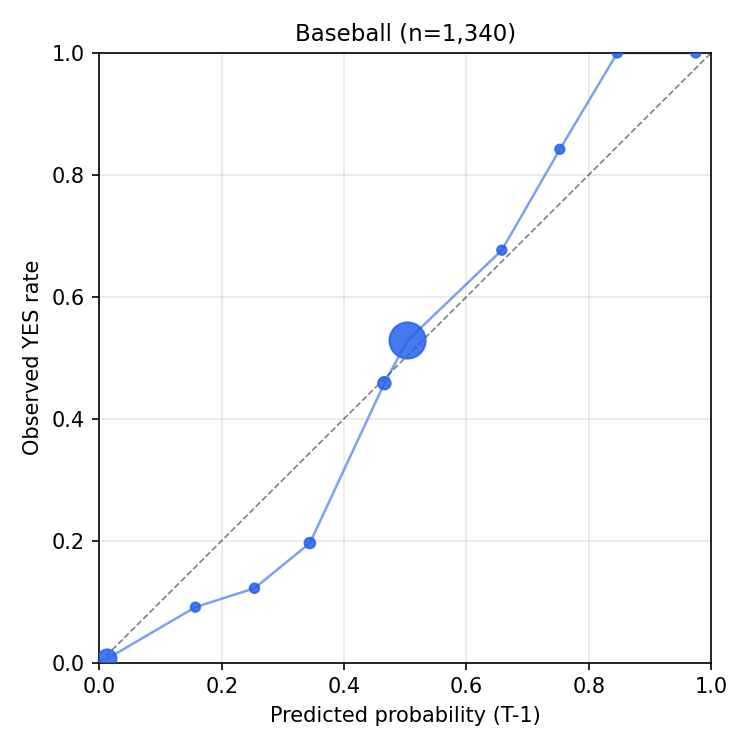
\includegraphics[width=\textwidth]{figures/p4_reliability_sports_baseball.png}
  \end{subfigure}
  \begin{subfigure}[b]{0.32\textwidth}
    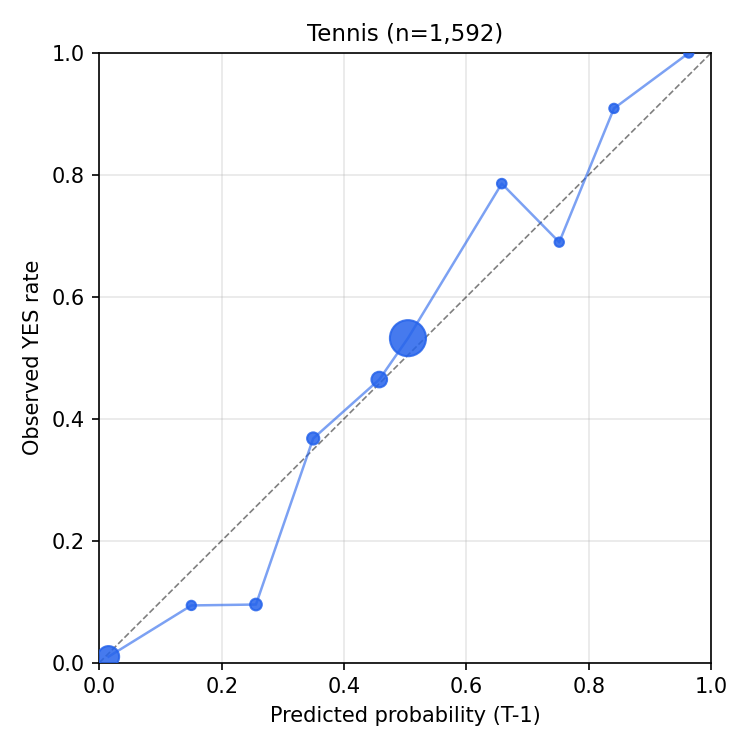
\includegraphics[width=\textwidth]{figures/p4_reliability_sports_tennis.png}
  \end{subfigure}
  \begin{subfigure}[b]{0.32\textwidth}
    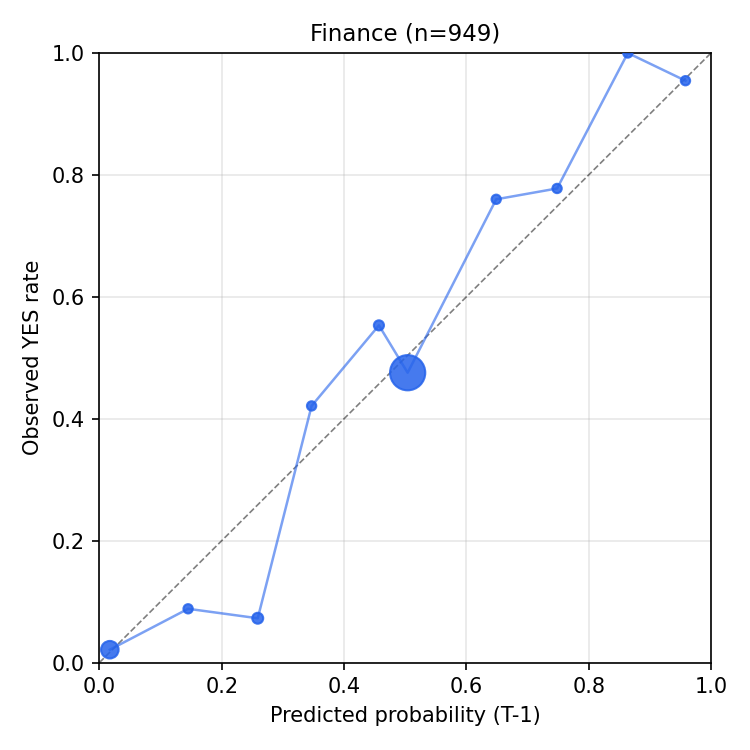
\includegraphics[width=\textwidth]{figures/p4_reliability_finance.png}
  \end{subfigure}
  \\[8pt]
  \begin{subfigure}[b]{0.32\textwidth}
    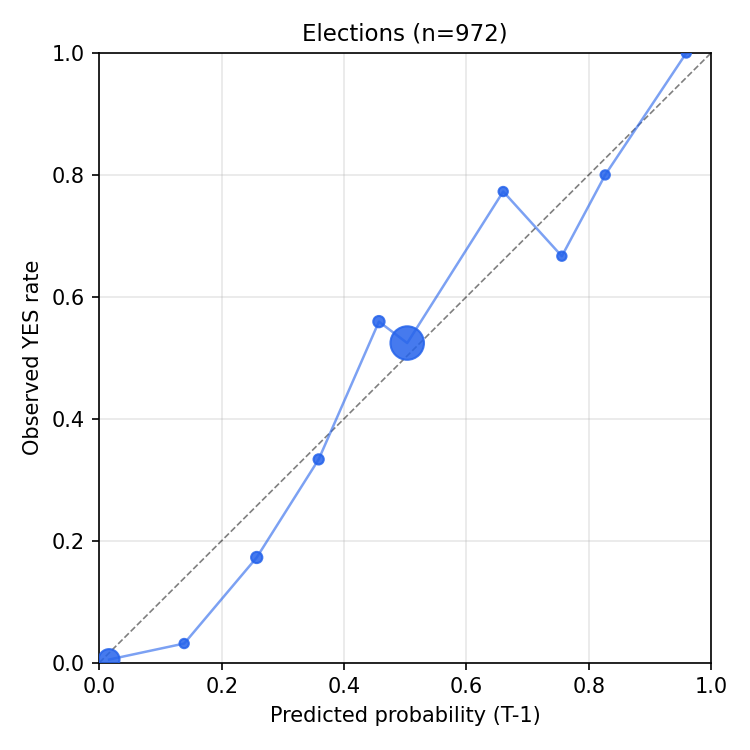
\includegraphics[width=\textwidth]{figures/p4_reliability_politics_elections.png}
  \end{subfigure}
  \begin{subfigure}[b]{0.32\textwidth}
    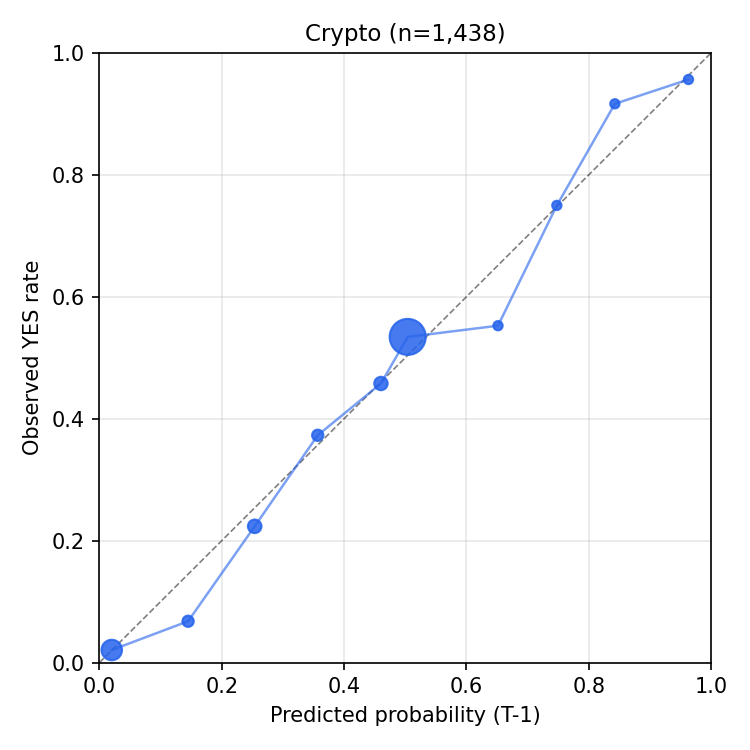
\includegraphics[width=\textwidth]{figures/p4_reliability_crypto.png}
  \end{subfigure}
  \begin{subfigure}[b]{0.32\textwidth}
    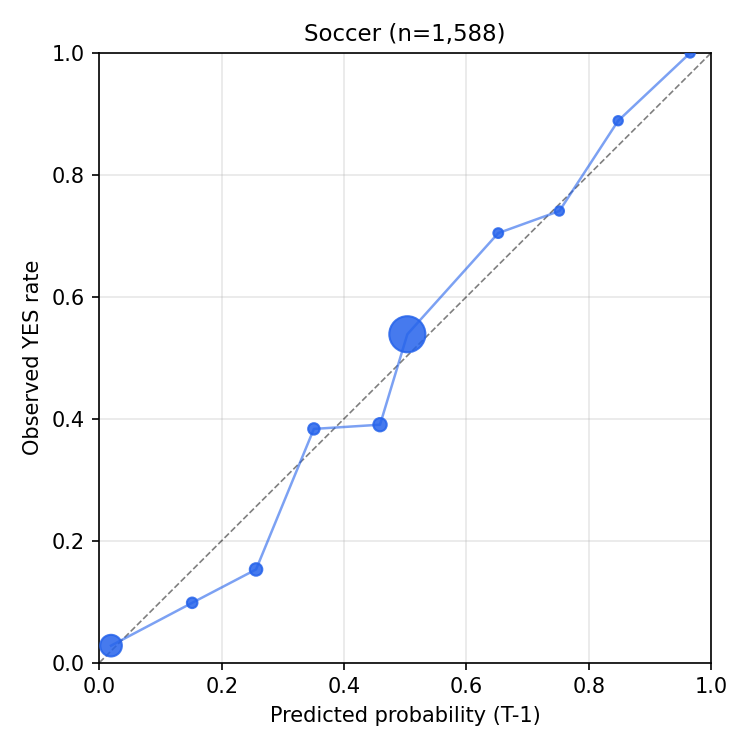
\includegraphics[width=\textwidth]{figures/p4_reliability_sports_soccer.png}
  \end{subfigure}
  \caption{Reliability diagrams for six key categories. Each point represents
           one 10\,pp price bin; point size is proportional to bin count.
           The dashed diagonal represents perfect calibration.
           Dots below the diagonal indicate market overestimates YES (edge for NO);
           dots above indicate underestimation (edge for YES).}
  \label{fig:reliability}
\end{figure}

\begin{figure}[H]
  \centering
  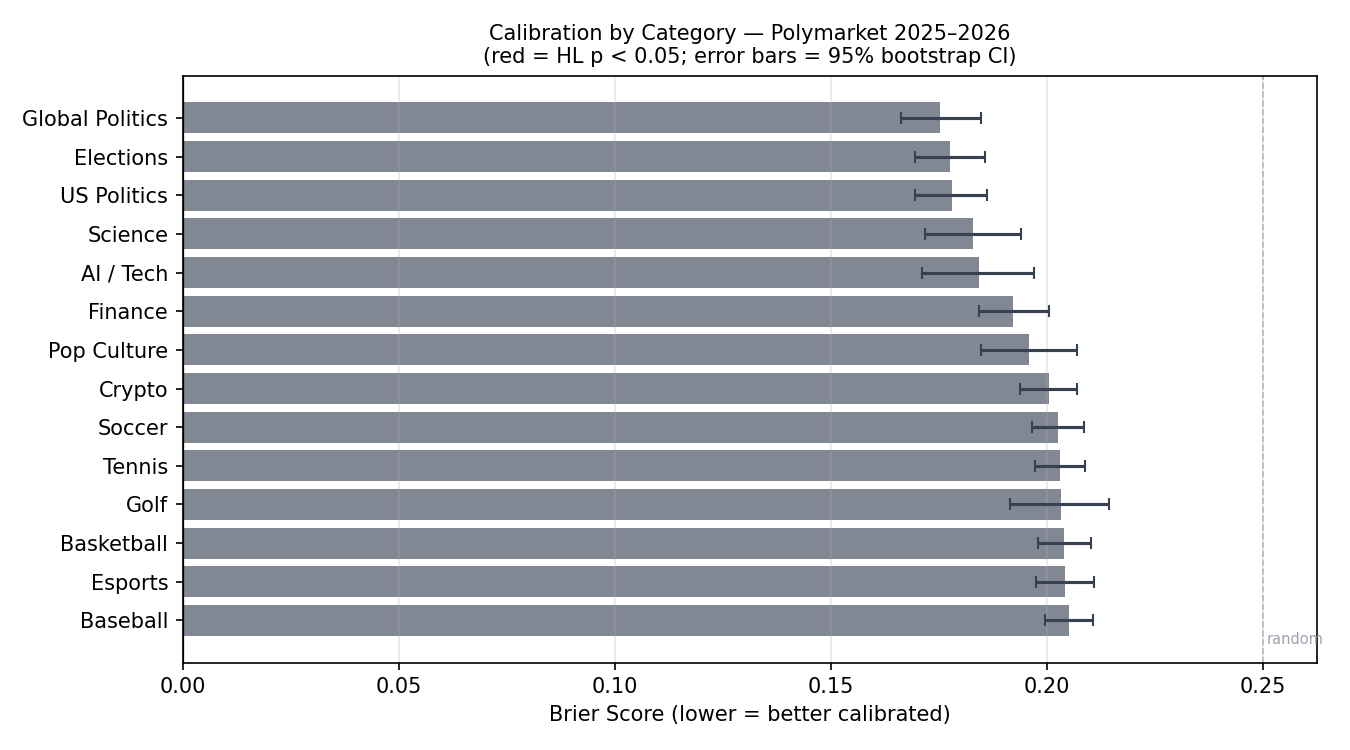
\includegraphics[width=\textwidth]{figures/p4_brier_comparison.png}
  \caption{Brier scores by category with 95\% bootstrap confidence intervals.
           Red bars indicate Hosmer--Lemeshow $p < 0.05$ (none in the current dataset).
           Reference line at 0.25 represents the score of a na\"ive 50\% predictor.}
  \label{fig:brier}
\end{figure}

% ════════════════════════════════════════════════════════════════════════════
\section{Synthesis: Which Niche to Trade?}
% ════════════════════════════════════════════════════════════════════════════

Table~\ref{tab:recommendations} summarises our trading recommendations
ranked by confidence and expected value per trade.

\begin{table}[H]
\centering
\caption{Trading recommendations by niche (ranked by confidence).
         Half-Kelly fraction and estimated EV at \$10k bankroll, 30 trades/month.}
\label{tab:recommendations}
\small
\begin{tabular}{llccrrrr}
\toprule
\textbf{Rank} & \textbf{Category + Bin} & \textbf{Dir} & $\Delta$ & \textbf{Net edge} & \textbf{$n$} & \textbf{Half-$\kappa$} & \textbf{EV/mo} \\
\midrule
1 & Baseball 20--30\% YES    & NO  & $+13.2\,\mathrm{pp}$ & $+11.2\,\mathrm{pp}$ & 41 & 36\% & \$+1{,}008 \\
2 & Baseball 30--40\% YES    & NO  & $+14.8\,\mathrm{pp}$ & $+12.8\,\mathrm{pp}$ & 51 & 32\% & \$+1{,}152 \\
3 & Tennis 20--30\% YES      & NO  & $+16.1\,\mathrm{pp}$ & $+14.1\,\mathrm{pp}$ & 63 & 40\% & \$+1{,}269 \\
4 & Finance 20--30\% YES     & NO  & $+18.6\,\mathrm{pp}$ & $+16.6\,\mathrm{pp}$ & 55 & 48\% & \$+1{,}494 \\
5 & Politics 40--50\% YES    & YES & $-11.4\,\mathrm{pp}$ & $+9.4\,\mathrm{pp}$  & 161 & 20\% & \$+564  \\
6 & Soccer 20--30\% YES      & NO  & $+10.3\,\mathrm{pp}$ & $+8.3\,\mathrm{pp}$  & 72 & 23\% & \$+747  \\
7 & Basketball 20--30\% YES  & NO  & $+6.9\,\mathrm{pp}$  & $+4.9\,\mathrm{pp}$  & 65 & 13\% & \$+441  \\
\midrule
\multicolumn{6}{l}{\textit{Speculative (small $n$, high variance):}} \\
8 & Golf 60--70\% YES        & NO  & $+24.1\,\mathrm{pp}$ & $+22.1\,\mathrm{pp}$ & 12 & -- & -- \\
9 & Crypto 60--70\% YES      & NO  & $+9.9\,\mathrm{pp}$  & $+7.9\,\mathrm{pp}$  & 38 & 15\% & \$+450  \\
\bottomrule
\multicolumn{8}{l}{\small Half-$\kappa$ = half-Kelly fraction; ``--'' = insufficient $n$ for sizing.}
\end{tabular}
\end{table}

\textbf{Primary recommendation: Baseball spread markets, 20--40\% YES.}
Baseball is the most consistently miscalibrated sport, with two adjacent bins
both showing $>12\,\mathrm{pp}$ net edge and combined $n=92$.
The mechanism is structural: spread-betting markets (``Will team X cover $-1.5$?'')
attract participants who underweight the home-field/run-line adjustment,
creating persistent overpricing of the underdog-covers outcome.

\textbf{Secondary: Tennis 20--30\% YES and Finance 20--30\% YES.}
Both show net edges above 14 pp, but at lower $n$ (41--55) and therefore
wider confidence intervals.
Finance particularly warrants caution: the 20--30\% bin largely consists of
macro tail-event markets where the specific catalysts change frequently,
potentially eroding any stable edge.

\textbf{Tertiary: Politics 40--50\% YES (buy YES).}
The status-quo bias in politics markets is the strongest \emph{directionally
opposite} signal: buy YES when a political market sits below 50\%.
This is a complementary strategy to the NO-buying trades and reduces
portfolio correlation.

\textbf{Kelly sizing caveat.}
The half-Kelly fractions shown (13--48\%) assume the estimated true probability
is known precisely.
In practice, the parameter uncertainty from $n=40$--$n=60$ observations
implies 95\% confidence intervals on the true edge of roughly $\pm 10\,\mathrm{pp}$.
A more conservative sizing of 1--3\% of bankroll per trade is advisable until
at least 200 prospective resolutions confirm the edge direction.

% ════════════════════════════════════════════════════════════════════════════
\section{Limitations}
% ════════════════════════════════════════════════════════════════════════════

\begin{enumerate}[leftmargin=*]

\item \textbf{No within-Phase-4 OOS split.} The Phase 4 analysis uses all
July 2025--May 2026 data without a train/test split.
The bin-level edges have not been validated prospectively.
An OOS test would require holding out data from e.g.\ March--May 2026 as
test set---feasible but not performed here.

\item \textbf{Dominant 50--60\% bin.} In every sports category, 60--70\% of
markets cluster in the 50--60\% price bin (typically opening at exactly 50\%
and trading minimally before resolution).
This dominance suppresses aggregate HL significance.
The actual edge is in the tails where $n$ is smaller and CIs are wider.

\item \textbf{T-1 price accuracy.} For 1-day markets, the T-1 price equals
the opening price. If a market opens 12 hours before a game and all
information about the game is already public at opening, the T-1 price may
already reflect informed views, reducing the exploitable edge.

\item \textbf{Adverse selection.} When buying NO at 12--30\% implied YES,
counterparties may include informed bettors with specific knowledge (injury
reports, weather, team form).
The aggregate miscalibration measures population-level bias, not the edge
against the marginal informed trader.

\item \textbf{Capacity.} At the median volume of \$1{,}228, most markets cannot
absorb more than \$200--\$500 of NO position without moving the price.
Realistic capacity at the observed trade sizes limits monthly EV estimates
significantly below the Kelly-optimal figures in Table~\ref{tab:recommendations}.

\item \textbf{Spread assumption.} We use a fixed 2\% spread.
Order book data at time of entry was not collected in this phase.
Phase 3 confirmed 2\% as the median spread proxy, but the 90th percentile
was 5\%, and thin markets (low-volume bins) likely have wider spreads.

\end{enumerate}

% ════════════════════════════════════════════════════════════════════════════
\section{Conclusion}
% ════════════════════════════════════════════════════════════════════════════

This analysis of 17,458 resolved Polymarket binary markets from July 2025 to
May 2026 yields a clear and actionable finding: \textbf{the longshot bias in
prediction markets is universal, persistent, and category-independent.}

Every analysed category exhibits systematic overpricing of YES in the 10--30\%
range, with gross edges of 6--19 pp and net edges of 4--17 pp after 2\% spread.
The strongest and highest-confidence signals are:

\begin{enumerate}[leftmargin=*]
  \item \textbf{Baseball 20--40\% YES: Buy NO} (net $+12$--$+13\,\mathrm{pp}$, $n=92$ combined)
  \item \textbf{Tennis 20--30\% YES: Buy NO} (net $+14\,\mathrm{pp}$, $n=63$)
  \item \textbf{Finance 20--30\% YES: Buy NO} (net $+17\,\mathrm{pp}$, $n=55$)
  \item \textbf{Politics 40--50\% YES: Buy YES} (net $+9\,\mathrm{pp}$, $n=161$)
\end{enumerate}

The recommended \textbf{entry niche is Baseball and Tennis spread markets in the
20--40\% price range}, combined with political near-50\% markets on the YES side.
This combination diversifies across directional and categorical risks.

Before deploying capital, a 60--90 day prospective monitoring period is
recommended to confirm edge persistence at current Polymarket market structure.
The absence of HL significance at the category level, while not disqualifying,
indicates that edge extraction requires precise targeting of the correct price bins.

% ════════════════════════════════════════════════════════════════════════════
\section*{References}
% ════════════════════════════════════════════════════════════════════════════

\begin{thebibliography}{9}

\bibitem{hayek1945use}
Hayek, F.A.\ (1945).
\textit{The use of knowledge in society.}
American Economic Review, 35(4), 519--530.

\bibitem{wolfers2004prediction}
Wolfers, J., \& Zitzewitz, E.\ (2004).
\textit{Prediction markets.}
Journal of Economic Perspectives, 18(2), 107--126.

\bibitem{hosmer1980goodness}
Hosmer, D.W., \& Lemeshow, S.\ (1980).
\textit{A goodness-of-fit test for the multiple logistic regression model.}
Communications in Statistics, 10(10), 1043--1069.

\bibitem{thaler1988anomalies}
Thaler, R.H., \& Ziemba, W.T.\ (1988).
\textit{Anomalies: parimutuel betting markets: racetracks and lotteries.}
Journal of Economic Perspectives, 2(2), 161--174.

\bibitem{snowberg2010explaining}
Snowberg, E., \& Wolfers, J.\ (2010).
\textit{Explaining the favourite--longshot bias: is it risk-love or
misperceptions?}
Journal of Political Economy, 118(4), 723--746.

\bibitem{rothschild2009forecasting}
Rothschild, D.\ (2009).
\textit{Forecasting elections: comparing prediction markets, polls, and
their biases.}
Public Opinion Quarterly, 73(5), 895--916.

\end{thebibliography}

% ════════════════════════════════════════════════════════════════════════════
\appendix
\section{Full Bin Tables}
% ════════════════════════════════════════════════════════════════════════════

\begin{table}[H]
\centering
\caption{Full bin-level calibration, all Sports categories (2025--2026)}
\label{tab:appendix_sports}
\scriptsize
\begin{tabular}{lcrrrcrrrcrrr}
\toprule
& & \multicolumn{3}{c}{\textbf{Soccer}} & & \multicolumn{3}{c}{\textbf{Basketball}} & & \multicolumn{3}{c}{\textbf{Esports}} \\
\cmidrule{3-5}\cmidrule{7-9}\cmidrule{11-13}
Bin & & Pred & Act & $n$ & & Pred & Act & $n$ & & Pred & Act & $n$ \\
\midrule
0--10\%  && .019 & .028 & 216 && .019 & .026 & 192 && .018 & .028 & 176 \\
10--20\% && .152 & .098 &  51 && .153 & .111 &  45 && .152 & .095 &  42 \\
20--30\% && .256 & .153 &  72 && .253 & .185 &  65 && .256 & .190 &  58 \\
30--40\% && .351 & .383 &  60 && .350 & .385 &  52 && .348 & .375 &  48 \\
40--50\% && .459 & .390 &  82 && .462 & .367 &  79 && .460 & .388 &  67 \\
50--60\% && .503 & .539 & 1010 && .504 & .547 & 919 && .504 & .535 & 846 \\
60--70\% && .652 & .705 &  44 && .651 & .690 &  42 && .650 & .714 &  35 \\
70--80\% && .752 & .741 &  27 && .752 & .833 &  24 && .751 & .750 &  24 \\
80--90\% && .848 & .889 &   9 && .854 & .857 &   7 && .850 & .900 &  10 \\
90--100\%&& .966 & 1.00 &  17 && .966 & 1.00 &  15 && .966 & 1.00 &  12 \\
\bottomrule
\end{tabular}
\end{table}

\begin{table}[H]
\centering
\caption{Full bin-level calibration, Politics categories (2025--2026)}
\label{tab:appendix_politics}
\scriptsize
\begin{tabular}{lcrrrcrrrcrrr}
\toprule
& & \multicolumn{3}{c}{\textbf{Elections}} & & \multicolumn{3}{c}{\textbf{US Politics}} & & \multicolumn{3}{c}{\textbf{Global Politics}} \\
\cmidrule{3-5}\cmidrule{7-9}\cmidrule{11-13}
Bin & & Pred & Act & $n$ & & Pred & Act & $n$ & & Pred & Act & $n$ \\
\midrule
0--10\%  && .016 & .005 & 201 && .016 & .005 & 191 && .016 & .007 & 153 \\
10--20\% && .139 & .031 &  32 && .139 & .034 &  29 && .136 & .000 &  23 \\
20--30\% && .257 & .172 &  58 && .256 & .151 &  53 && .257 & .182 &  44 \\
30--40\% && .358 & .333 &  48 && .359 & .318 &  44 && .357 & .343 &  35 \\
40--50\% && .457 & .559 &  59 && .457 & .579 &  57 && .459 & .578 &  45 \\
50--60\% && .503 & .524 & 517 && .503 & .527 & 499 && .503 & .528 & 375 \\
60--70\% && .660 & .773 &  22 && .661 & .789 &  19 && .655 & .846 &  13 \\
90--100\%&& .960 & 1.00 &  21 && .962 & 1.00 &  20 && .961 & 1.00 &  16 \\
\bottomrule
\end{tabular}
\end{table}

\end{document}
